% https://en.wikipedia.org/wiki/Succinct_data_structure
\chapter{Strutture dati succinte}
Le \textbf{strutture dati succinte} sono una classe di strutture dati che forniscono
un compromesso tra l'efficienza dell'accesso ai dati e la quantità di spazio
utilizzato per memorizzare i dati. Queste strutture cercano di minimizzare l'uso
dello spazio di memoria, mantenendo nel contempo un accesso efficiente ai dati.

Le strutture dati succinte sono un tipo di struttura dati che utilizza una quantità
di spazio “vicina” al limite inferiore teorico dell'informazione, ma che, a
differenza di altre rappresentazioni compresse, consente ancora operazioni di
interrogazione efficienti.

Supponiamo che $\mathcal{Z}$ sia il numero ottimale teorico di bit necessari per
memorizzare alcuni dati. Una rappresentazione di questi dati viene chiamata:
\begin{itemize}
    \item \textbf{Implicita} se richiede $\mathcal{Z} + \mathcal{O}(1)$ bit di
          spazio. (es. $\mathcal{Z} + 14$ bit)
    \item \textbf{Succinta} se richiede $\mathcal{Z} + o(\mathcal{Z})$ bit di spazio.
          (es. $\mathcal{Z} + \log \mathcal{Z}$ oppure $\mathcal{Z} + \sqrt{
                  \mathcal{Z}}$ bit)
    \item \textbf{Compatta} se richiede $\mathcal{O}(\mathcal{Z})$ bit di spazio.
          (es. $5 \cdot \mathcal{Z}$ bit)
\end{itemize}
\begin{nota}
    $o(\mathcal{Z})$ si riferisce al concetto matematico di \textit{o-piccolo},
    ovvero:
    \begin{equation}
        \lim_{x \to x_0} \frac{f(x)}{g(x)} = 0 \Rightarrow f(x) = o_{x_0} (g(x))
        \ \text{con} \ x_0 = + \infty
    \end{equation}
\end{nota}
\section{Bitvector}
Un modo di rappresentare le strutture dati succinte è attraverso l'utilizzo di
\textbf{bitvector}.
\begin{definizione}[\textbf{Bitvector}]
    Si definisce un \textbf{bitvector} $B$ come un array di lunghezza $n$, popolato
    da elementi binari ($\{0, 1\}$). Formalmente si ha:
    \begin{equation}
        B[i] \in \{0, 1\}, \ \forall i \ \text{tale che} \ 1 \leq i \leq n
    \end{equation}
    In alternativa all'alfabeto binario è possibile utilizzare i valori booleani
    vero e falso ($\{\top, \bot\}$).
\end{definizione}
Su questa struttura è possibile effettuare due operazioni:
\begin{itemize}
    \item \textbf{rank}: restituisce il numero di elementi uguali a $q$ che sono
          presenti nella struttura dati fino a $x$.
          \begin{equation}
              rank_q(x) = \sum_{k = 1}^{k \leq x} B[k], \ \forall x \
              \text{tale che} \ 1 \leq x \leq n \ \land \ B[k] = q
          \end{equation}
    \item \textbf{select}: restituisce la posizione della $x$-esima occorrenza
          di $q$.
          \begin{equation}
              select_q(x) = \min{\{k \in [0, \dots, n): \ rank_q(k) = x\}}
          \end{equation}
\end{itemize}
\begin{nota}
    \begin{equation}
        rank_q(select_q(i)) = i
    \end{equation}
\end{nota}
È possibile ottenere una struttura dati succinta, usando $o(n)$ bit aggiuntivi,
che permetta di effettuare le operazioni di \textit{rank} e \textit{select} in
tempo costante $\mathcal{O}(1)$.
\subsection{Funzione rank}
Vediamo ora come è possibile rendere il tempo di esecuzione dell'operazione di
rank costante ($\mathcal{O}(1)$).

La soluzione più semplice, ovvero memorizzare tutti i valori di $rank(i)$
necessiterebbe di $\mathcal{O}(n \log n)$ bit il che non lo rende un o-piccolo
di $n$. Una soluzione alternativa consiste nel memorizzare ogni $l-$esimo valore
$rank(i)$, e a questo punto, quando si esegue una query scorriamo i restanti $l
    - 1$ bit.

Questi valori vengono salvati in un vettore \textit{first} $F[0 \dots n / l]$,
dove l'operatore $/$ indica la divisione intera, tale che:
\begin{itemize}
    \item $F[0] = 0$
    \item $F[i / l] = rank(i)$ se $i \mod l = 0$
\end{itemize}
Se $l = \left(\left\lceil \frac{\log n}{2} \right\rceil \right)^2$ si ha un ordine
di $\frac{n}{\log n}$ bit per l'array $F$. Con questa prima operazione è possibile
eseguire una rank come:
\begin{equation}
    rank(i) = F[i/l] + C(B[l \cdot (i / l) + 1 \dots i])
\end{equation}
con $C(B')$ che rappresenta una funzione che conta i simboli $\sigma = 1$ in $B'$.
Questa soluzione mi porta a una rank eseguita in tempo $\mathcal{O}(\log^2 n)$.

Aumentando la quantità di informazioni salvate in memoria, possiamo ridurre
ulteriormente il tempo di esecuzione della funzione di rank.

Nello specifico, in ogni blocco di lunghezza $l$, indotto da $F$, memorizziamo
ogni $k$ posizioni il numero di simboli $\sigma = 1$ a partire dall'inizio del
blocco, escludendo la posizione iniziale in cui il valore di rank è già in $F$.
Otteniamo un vettore \textit{second} $S[0 \dots l /k]$ dove:
\begin{itemize}
    \item $S[i / k] = 0$ se $k \mod l = 0$
    \item $S[i / k] = rank_{B[l \cdot (i / l) + 1 \dots i]} (i - l \cdot (i / l)
              + 1)$ se $i \mod k = 0$
\end{itemize}
Questa soluzione richiede $\mathcal{O}\left(\left(\frac{n}{k}\right) \log l\right)$
bit aggiuntivi. In particolare, scegliendo $k = \left\lceil \frac{\log n}{2}
    \right\rceil$ si ottiene uno spazio di $\mathcal{O}(\frac{n \log \log n}{\log n})$
bit. Introducendo questo secondo vettore è possibile eseguire una rank come:
\begin{equation}
    rank(i) = F[i / l] + S[i / k] + C(B[k \cdot (i / k) + 1 \dots i])
\end{equation}
Questa soluzione mi porta a una rank eseguita in tempo $\mathcal{O}(\log n)$.

Per ottenere una rank in tempo costante si utilizza la tecnica \textbf{Four
    Russians technique}. Questa tecnica consiste nel salvare una look-up table
third $T$, di dimensioni $2^{k - 1} \times k - 1$, i valori di $rank(i')$
per tutte le posizioni $k - 1$, in tutte le possibili configurazioni indotte dai
blocchi definiti per $S$. Così facendo la lookup-table $T$ richiede uno spazio
per essere memorizzata pari a $\mathcal{O}(\sqrt{n} \log n \log \log n)$ bit.

Si definisce:
\begin{equation}
    c_i = B \left[k \cdot \left(\frac{i}{k}\right) + 1 \dots k \cdot \left(\frac{i}{k} 
    + 1\right) - 1\right]
\end{equation}
come il bitvector di lunghezza $k - 1$ che copre il $(k + 1)-$esimo blocco. Questo
valore ci permette di identificare la riga della lookup table $T$ da cui prendere
il valore di $rank(i)$. Mentre la colonna si ottiene da $i \mod k$. In questo
modo è possibile eseguire una rank in tempo costante $\mathcal{O}(1)$.
\begin{equation}
    rank(B) = \begin{cases}
        F[i/l]                                   & \text{se} \ i \mod l = 0    \\
        F[i/l] + S[i/k]                          & \text{se} \ i \mod l \neq 0
        \land i \mod k = 0                                                     \\
        F[i/l] + S[i/k] + T[c_i][(i \mod k) - 1] & \text{se} \ i \mod l \neq 0
        \land i \mod k \neq 0                                                  \\
    \end{cases}
\end{equation}
Così facendo, memorizzando un $o(n)$ bit in aggiunta alla struttura, posso
eseguire l'operazione di rank in tempo costante.
\begin{nota}
    Le operazioni per arrivare alla costruzione delle struttura dati che mi
    permette di eseguire la rank in tempo costante sono eseguite in tempo lineare
    ($\mathcal{O}(n)$).
\end{nota}
\begin{esempio}
    Vediamo un esempio di come può essere implementata la funzione rank in modo
    da effettuare accesso in tempo costante. Consideriamo il bitvector
    $B = 100101010010$ e scegliamo i valori di $l = 9$ e $k = 3$. Per eseguire
    la funzione rank in tempo costante si ottiene la struttura riportata in
    figura \ref{fig:rank}.
    \begin{figure}[!ht]
        \centering
        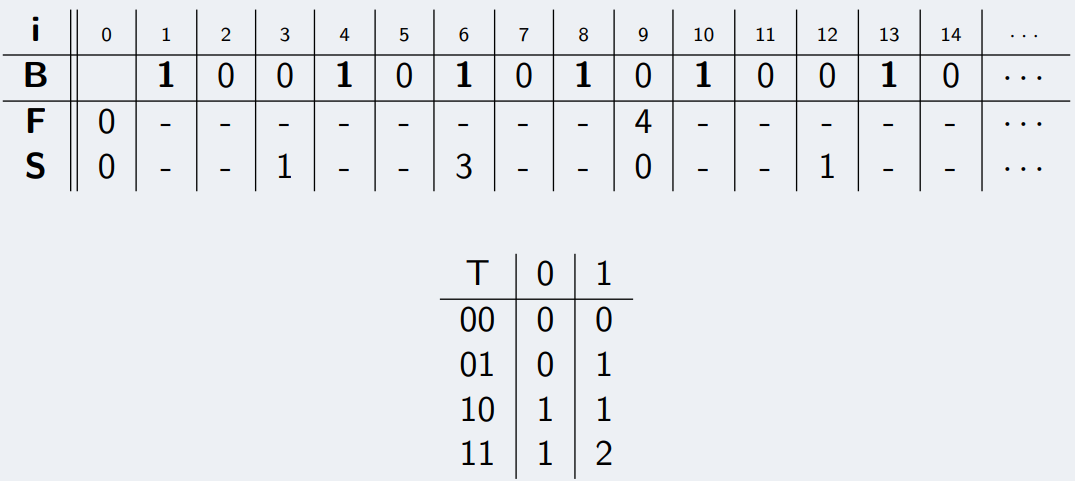
\includegraphics[width=0.5\textwidth]{img/Strutture Dati/rank.png}
        \caption{Esempio di implementazione della funzione rank}
        \label{fig:rank}
    \end{figure}
\end{esempio}
\begin{osservazione}
    Si può dimostrare che, con un procedimento abbastanza analogo a quello visto
    per la funzione di rank, è possibile costruire una struttura che necessita di
    $o(n)$ bit aggiuntivi e che permette di effettuare l'operazione di select in
    tempo costante.
\end{osservazione}
\section{Level Order Unary Degree Sequence}
Consideriamo in memoria la rappresentazione di un albero etichettato con $n$ nodi.
La classica rappresentazione attraverso puntatori richiede uno spazio pari a
$\mathcal{O}(n \log n)$.

Analizziamo ora una rappresentazione basata sulla visita in left-to-right
level-order di un albero, ovvero una visita in ampiezza. Utilizzando questa
visita, si salva per ogni nodo il suo grado e si memorizza la sequenza dei gradi
$D$ attraverso un prefix code binario. Quindi, per ogni nodo si aggiunge a un
bitvector $B$ i simboli della sequenza $1^d0$, con $d$ che rappresenta il grado.

In questa rappresentazione si considera un nodo detto \textbf{super-root}, il
quale viene aggiunto in modo che il numero di valori uguali a 1 presenti nel
bitvector sia uguale al numero di nodi dell'albero.

In questo modo si arriva a ottenere un bitvector di lunghezza $2n + 1$ dove si
ha un simbolo 1 associato a ogni nodo dell'albero. Con questa rappresentazione
posso indicare il nodo $m$ con l'indice relativo del corrispondente bit 1.

Utilizzando le operazioni rank e select definite per il bitvector, è possibile
implementare un set di operazioni per interrogare questa rappresentazione
dell'albero.
\begin{itemize}
    \item $is\_leaf(v) = T$ se e solo se $select_0(v) = select_0(v + 1) - 1$ in
          quanto per costruzione una foglia aggiunge solo uno 0 al bitvector $B$,
          quindi con $select_0(v)$ troviamo la posizione dello 0 posto in $B$ dal
          nodo antecedente a $v$ nella visita (quello antecedente perché abbiamo
          il 10 della super-root) e con $select_0(v + 1)$ la posizione dello 0
          relativo a $v$. Se sono in due posizioni adiacenti significa che $v$ ha
          aggiunto solo uno $0$ e quindi è una foglia.
    \item $first\_child(v) = rank_1(select_0(rank_1(select_1(v)))+1) = rank_1
              (select_0(v)+1)$:
          \begin{itemize}
              \item $k = select_0(v) + 1$ restituisce la posizione $k$ su $B$ del
                    primo "figlio" di $v$. In altri termini il $v$-esimo 0 mi
                    dice che ho finito di "visitare" la sotto-sequenza di bitvector
                    costruita per il nodo $v - 1$ e al bit successivo inizia la
                    sequenza del bitvector per $v$.
              \item $m = rank_1(k)$ restituisce il numero di nodo dell'albero in
                    posizione $k$ di $B$, quindi la label del primo "figlio" di
                    $v$.
              \item Imponiamo che $first\_child(v) = - 1$ se $is\_leaf (v) = T$
          \end{itemize}
    \item $last\_child(v) = rank_1(select_0(rank_1(select_1(v))+1)-1) = rank_1
              (select_0(v+1)-1)$:
          \begin{itemize}
              \item $k = select_0(v + 1)$ restituisce la posizione $k$ su $B$
                    dello $0$ inserito in visita level-order del nodo con label
                    $v$. In altri termini, il (v + 1)-esimo 0 mi dice che ho
                    finito di "visitare" la sotto-sequenza di bitvector costruita
                    per il nodo $v$.
              \item $w = k - 1$ restituisce l'indice dell'ultimo 1 inserito in
                    visita level-order del nodo con label j, quindi l'indice su
                    B dell'ultimo "figlio" di c. In altri termini, con la
                    precedente operazione si raggiunge lo 0 di $1^d 0$ e col -1
                    l'ultimo 1 di $1^d$
              \item $m = rank_1(w)$ restituisce il numero di nodo dell'albero in
                    posizione $w$ di B, quindi la label dell'ultimo "figlio" di v.
              \item Imponiamo che $last\_child(v) = -1$ se $is\_leaf (v) = T$
          \end{itemize}
    \item $parent(v) = rank_1(select_1(rank_0(select_1(v)))) = rank_0(select_1(v))$:
          \begin{itemize}
              \item $i = select_1(v)$ restituisce la posizione $i$ del nodo $v$
                    nel bitvector $B$ (identificando in quale $1^d 0$ è stato
                    aggiunto).
              \item $j = rank_0(i)$ restituisce il numero di sequenze che sono
                    state aggiunte al bitvector $B$ fino a quella relativa al
                    "genitore" del nodo in posizione $i$. Il numero di tali
                    sequenza è l'indice del nodo "genitore" per definizione di
                    vista level order e conseguente etichettatura dei nodi.
              \item Imponiamo che $parent(v) = -1$ se $v = 1$ (non considero la
                    super-root)
          \end{itemize}
    \item $degree(v) \ = \ last\_child(v) - first\_child(v) + 1$, imponiamo 
          $degree(v) = 0$ se $last\_child(v) = first\_child(v) = -1$
    \item $nth\_child(v, nth) = rank_1(select_1(first\_child(v)) + nth - 1)$,
          imponiamo $nth\_child(v, nth) = -1$ se $degree(v) < nth$
\end{itemize}
\begin{esempio}
    In figura \ref{fig:louds}, è riportata la costruzione di un e Level Order
    Unary Degree Sequence.
    \begin{figure}[!ht]
        \centering
        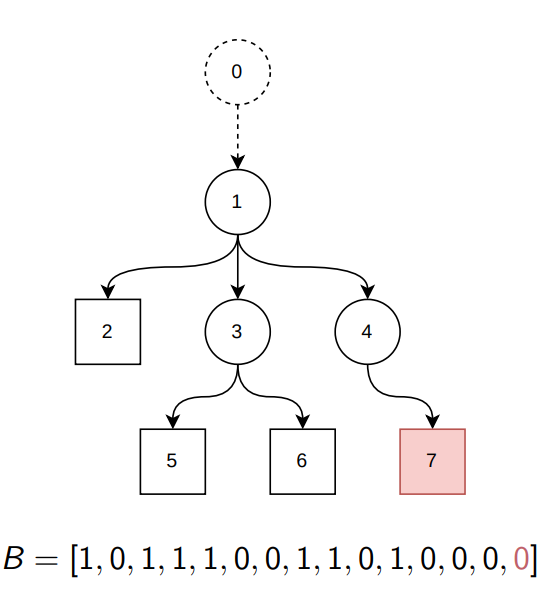
\includegraphics[width=0.5\textwidth]{img/Strutture Dati/LOUDS.png}
        \caption{Esempio di costruzione di un e Level Order Unary Degree Sequence}
        \label{fig:louds}
    \end{figure}
\end{esempio}
\section{Wavelet Tree}
Abbiamo visto come rank e select possono essere usati per interrogare un bitvector,
che ha un alfabeto fisso di grandezza 2. Siamo ora interessati a generalizzare
tali query ad un alfabeto di grandezza arbitraria. Per praticità assumiamo di
avere un alfabeto $\Sigma = [1 \dots s]$ il quale è ordinato nel seguente modo:
\begin{equation}
    \Sigma[i] \prec \Sigma[j] \iff i < j \dots
\end{equation}
Dato un generico alfabeto $\Sigma$ e una sequenza $T[1\dots n] \in \Sigma$ possiamo
ri-definire le funzioni di rank e select come:
\begin{itemize}
    \item $rank_{\sigma,T} (i)$ conta tutte le occorrenze del simbolo $\sigma
              \in \Sigma$ fino all'indice $i$ in $T$, $i \leq | T |$.
    \item $select_{\sigma,T} (i)$ ritorna la posizione dell'i-esima occorrenza
          del simbolo $\sigma \in \Sigma$ in $T$, $i \leq | T |$.
\end{itemize}
\begin{equation}
    rank_{\sigma,T} (select_{\sigma,T} (i)) = i, \ \forall \sigma \in \Sigma
    \land \forall i = 1 \dots n
\end{equation}

Una rappresentazione ``naïve'' consiste nel considerare come rappresentazione di
$T$ attraverso un insieme di $s$ ($| \Sigma | = s$) stringhe binarie $B_\sigma[1
        \dots n]$, $\forall \sigma \in \Sigma$, ovvero una per ogni simbolo
dell'alfabeto, si ha che:
\begin{equation}
    B_\sigma[i] = \begin{cases}
        1 \iff T[i] = \sigma \\
        0 \iff T[i] \neq \sigma
    \end{cases}
\end{equation}
Se per ogni bitvector $B_\sigma$ abbiamo calcolato la struttura a supporto vista
precedentemente si ha $rank_{\sigma,T} (i)$ in tempo costante $\mathcal{O}(1)$ e
uno spazio pari a $s \cdot (n + o(n))$ bit aggiuntivi.

Possiamo ottenere una rappresentazione più efficiente in memoria senza sacrificare
troppo i tempi di query. Per realizzare questa rappresentazione consideriamo un
\textbf{albero binario perfettamente bilanciato} dove ogni nodo corrisponde ad un
sottoinsieme di $\Sigma$.

I due figli di ogni nodo partizionano il corrispondente sottoinsieme di $\Sigma$
in due. A ogni nodo $v$ corrisponde una sequenza chiamata $R_v$, la quale è una
sotto-sequenza dell'input $T$ ed è anche una sotto-sequenza della sequenza con
cui è etichettato il nodo genitore di $v$. La root corrisponde alla sequenza $R_v = T$.

A ogni nodo $v$ si associa un bitvector, denotato con $B_v$, che indica a quale
dei due figli del nodo $v$ ogni simbolo della sotto-sequenza $R_v$ appartiene.

Se consideriamo l'indice $j$, con $1 \leq j \leq |R_v|$, abbiamo che:
\begin{itemize}
    \item Se $B_v [j] = 0$, allora il carattere associato $R_v [j]$ appartiene
          alla sotto-sequenza rappresentata dal figlio di sinistra.
    \item Se $B_v [j] = 1$, allora il carattere associato a $R_v [j]$ appartiene
          alla sotto-sequenza rappresentata dal figlio di destra.
\end{itemize}
Le foglie dell'albero sono \textit{virtualmente} etichettate con i singoli
caratteri dell'alfabeto. In realtà ci basta la funzione $rank_1$ eseguita sui
bitvector che etichettano i genitori delle foglie per recuperare l'informazione.
\subsection{Operazioni}
Vediamo ora come realizzare le operazioni su questa struttura dati:
\begin{itemize}
    \item \textbf{rank}: il calcolo dell'operazione rank inizia nel nodo root,
          nel quale si determina a quale dei due figli appartiene $\sigma$.
          Questa operazione avviene utilizzando l'ordinamento dell'alfabeto. In
          particolare, nella radice se $B_v [j] = 0$ allora $R_v [j] = \Sigma
              \left[\left\lceil \frac{s}{2} \right\rceil\right] \lor R_v [j]
              \prec \Sigma \left[\left\lceil \frac{s}{2} \right\rceil\right]$,
          ovvero il carattere si trova nella prima metà dell'alfabeto. Altrimenti
          se $B_v[j] = 1$ allora il carattere che si cerca è nella seconda metà
          dell'alfabeto.

          A questo punto si prosegue nel seguente modo fino a raggiungere le foglie:
          \begin{itemize}
              \item Se $\sigma = \Sigma\left[\left\lceil \frac{s}{2} \right\rceil
                            \right] \lor \sigma \prec \Sigma\left[\left\lceil
                            \frac{s}{2} \right\rceil\right]$ (siamo nella prima
                    metà dell'alfabeto indotto dal nodo), allora si prosegue
                    verso il figlio di sinistra, aggiornando il valore di $i$ con
                    $i = rank_{0,B_v}(i)$.
              \item Altrimenti, ovvero se siamo nella seconda metà, usiamo il
                    figlio di destra, e aggiorniamo il valore di $i$ con $i =
                        rank_{1,B_v}(i)$.
          \end{itemize}
          Nel nuovo nodo $v$ si procede nello stesso modo, considerando che ora
          $\Sigma = \Sigma \left[1 \dots \left\lceil \frac{s}{2} \right\rceil\right]$
          se si è andati a sinistra e $\Sigma = \Sigma\left[\left\lceil
                  \frac{s}{2} \right\rceil + 1 \dots s\right]$ se si è andati a
          destra.

          Si prosegue fino ad una foglia e $rank_{\sigma,T} (i) = i'$, dove $i'$
          è l'ultimo valore di i che si ottiene nei vari step.

          L'albero ha altezza $\lceil \log s\rceil$ quindi $rank_{\sigma,T} (i)$
          può essere calcolato in $\mathcal{O}(\log s)$, dove $s$ è la cardinalità
          dell'alfabeto.
    \item \textbf{random access}: in questo caso la scelta del figlio dipende
          unicamente da $B_v [i]$:
          \begin{itemize}
              \item Se $B_v [i] = 0$ proseguo verso il "figlio" di sinistra,
                    con $i = rank_{0,B_v}(i)$
              \item Se $B_v [i] = 1$ proseguo verso il "figlio" di destra,
                    con $i = rank_{1,B_v}(i)$
          \end{itemize}
          Si prosegue fino ad una foglia scegliendo il percorso da seguire in
          base al valore di $B_v [i]$.

          $T[i]$ è il simbolo che etichetta la foglia raggiunta alla fine della
          visita dato che il wavelet tree di una sequenza $T$ garantisce random
          access alla sequenza stessa possiamo sostituirla col suo wavelet tree.

          L'albero ha altezza $\lceil\log s \rceil$ quindi $access_{\sigma,T} (i)$
          può essere calcolato in $\mathcal{O}(\log s)$.
    \item \textbf{select}: analogamente ai bitvector si può dimostrare che anche
          $select_{\sigma,T}(i)$ può essere calcolato in $\mathcal{O}(\log s)$
\end{itemize}
\begin{nota}
    Nell'operazione di access ad ogni passo si effettua l'operazione di rank
    in base al valore del bit $B_v [i]$. Quindi per ogni nodo si effettua una
    scelta se effettuare una rank sul valore $0$ o sul valore $1$.
\end{nota}
\subsection{Costruzione}
Vediamo ora come costruire un wavelet tree livello per livello a partire dalla
root:
\begin{enumerate}
    \item Si etichetta la root con $R_v = T$ e un bitvector $B_v$ tale che
          $\forall i$, con $1 \leq i \leq |T|$:
          \begin{equation}
              B_v[i] = \begin{cases}
                  0 \iff T[i] = \Sigma\left[\left\lceil \frac{s}{2}
                      \right\rceil\right] \lor T[i] \prec \Sigma\left[
                  \left\lceil \frac{s}{2} \right\rceil\right] \\
                  1 \text{ altrimenti}
              \end{cases}
          \end{equation}
    \item Si estrae la sotto-sequenza $T'$ corrispondente ai valori 0 di $B_v$ e
          la si usa per etichettare il ``figlio'' di sinistra $v_1$ (che è relativo
          all'alfabeto $\Sigma = \Sigma\left[1 \dots \left\lceil \frac{s}{2}
                  \right\rceil\right]$) mentre quella corrispondente ai valori 1
          la si usa per etichettare il ``figlio'' di destra $v_2$ (che è relativo
          all'alfabeto $\Sigma = \Sigma\left[\left\lceil \frac{s}{2} \right\rceil
                  + 1 \dots s \right]$) per entrambe.
    \item Posso quindi cancellare $T$ e costruire i bitvector $B_{v1}$ e $B_{v2}$,
          con le rispettive strutture per la funzione rank e continuare
          ricorsivamente fino al raggiungimento delle foglie (quando si
          raggiungono alfabeti di cardinalità 1).
\end{enumerate}
Il processo di costruzione di un wavelet tree richiede un tempo pari a
$\mathcal{O}(n \log s)$.

In ogni momento della costruzione del wavelet tree abbiamo un bound in spazio
pari a $3n \log s + \mathcal{O}(s \log n)$, dato da:
\begin{itemize}
    \item 3 sotto-sequenze di $T$, quella del "genitore" e quelle dei due "figli".
    \item Tutti i bitvector finora computati che formano il wavelet tree.
    \item I puntatori che memorizzano la struttura ad albero.
\end{itemize}
Un ulteriore miglioramento in spazio si può ottenere concatenando tutti i bitvector
in un unico bitvector con una sola struttura a supporto della funzione rank. In
tal caso la struttura ad albero si può inferire dai partizionamenti dell'alfabeto
e dai bitvector. Questa variante è chiamata \textbf{levelwise wavelet tree}.

Un wavelet tree per una sequenza lunga $n$ costruita su alfabeto di cardinalità
$s$ occupa, avendo $\mathcal{O}(s \log n)$ per la topologia dell'albero:
\begin{equation}
    n \log s + o(n \log s) + \mathcal{O}(s \log n) \ bit
\end{equation}
Mentre, un levelwise wavelet tree richiede:
\begin{equation}
    n \log s + o(n \log s) \ bit
\end{equation}
\begin{esempio}
    Costruzione di un wavelet tree:
    \begin{figure}[!ht]
        \centering
        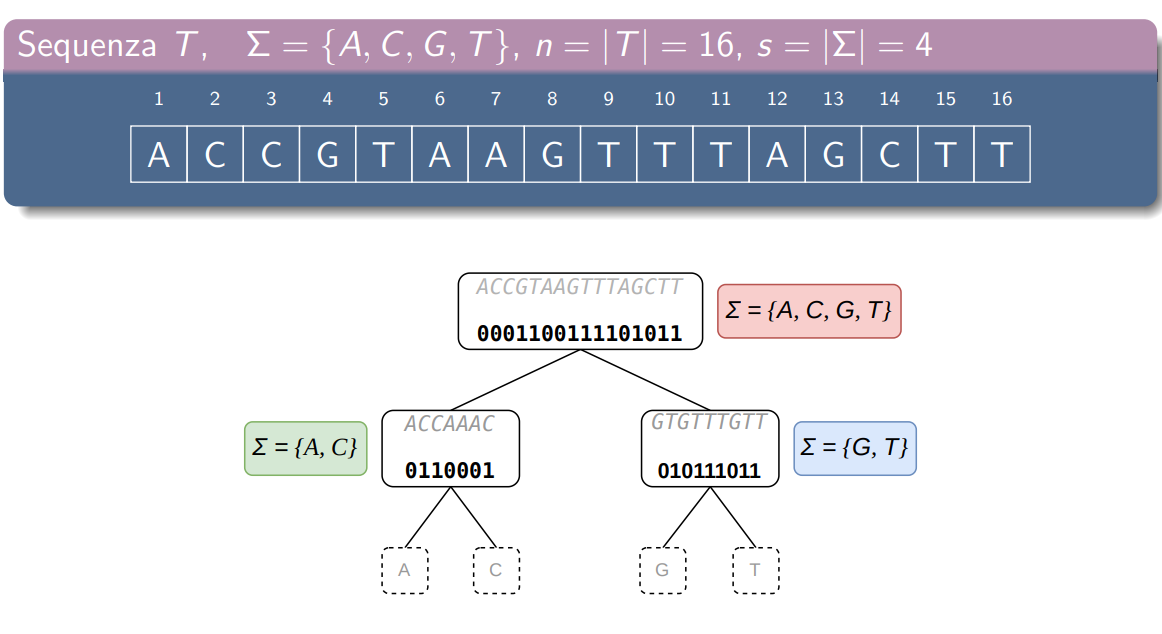
\includegraphics[width=0.5\textwidth]{img/Strutture Dati/wavelet tree.png}
        \caption{Esempio di costruzione di un wavelet tree su una sequenza semplice}
    \end{figure}
\end{esempio}
\section{Altre strutture dati succinte}
\begin{itemize}
    \item \textbf{Parentesi bilanciate}: si costruisce a partire dalla DFS
          dell'albero (preorder):
          \begin{itemize}
              \item ``('' quando si raggiunge un nodo per la prima volta.
              \item ``)'' quando si è terminata la visita del sotto-albero.
          \end{itemize}
    \item Strutture dati succinte che supportano le \textbf{range minimum queries}.
    \item \textbf{Wavelet matrix}: nascono con l'idea di migliorare i levelwise
          wavelet tree nella gestione di larghi alfabeti:
          \begin{itemize}
              \item tempi di access dimezzati
              \item tempi di rank e select leggermente ridotti
          \end{itemize}

          L'idea è che i bit di un nodo "figlio" non sono più "allineati" al
          "genitore" ma si assume che passando da un livello all'altro, tutti gli
          zero vanno da una parte e gli uni dall'altra.

          Salvando ad ogni livello $l$ il numero totale di simboli $\sigma = 0$
          $z_l$, richiedendo in totale $\mathcal{O}(\log n \log s)$ bit, si ottiene
          lo stesso comportamento di un levelwise wavelet tree.

          Una wavelet matrix richiede $n \log s + o(n \log s)$ bit, può essere
          costruita in $\mathcal{O}(n \log s)$ e risponde alle stesse query di un
          (levelwise) wavelet tree in $\mathcal{O}(\log s)$
\end{itemize}
\begin{definizione}[\textbf{Range Minimum Query}]
    Dato un array $A[1\dots n]$ di numeri $n$ elementi da un universo totalmente
    ordinato la \textbf{Range Minimum Query} $RMQ_A(i, j)$, con $1 \leq i \leq
        j \leq n$, restituisce la posizione $k$ di un elemento minimo in $A[i
                \dots j]$:$$RMQ_A(i, j) = argmin_{i \leq k \leq j}\{A[k]\}$$

    Si può dimostrare che è possibile costruire una struttura dati succinta che
    richiede $2n + o(n)$ bit in memoria e che risponde in $\mathcal{O}(1)$.
\end{definizione}
\chapter{Strutture Dati Probabilistiche Hashing-Based}
Su strutture dati semplici come array, matrici, etc$\dots$ posso eseguire operazioni
di accesso, cancellazione di un elemento e inserimento di un elemento in tempo
$\mathcal{O}(1)$ data la chiave $k$, l'input $x$ e la posizione $k[x]$.

Con queste strutture dati si ha un problema in quanto è possibile che l'insieme
delle chiavi utilizzate sia molto minore rispetto alla dimensione della struttura
dati. Una soluzione a questo problema sono le \textbf{hash tables}.

Se con l'accesso diretto l'elemento con chiave $k$ era memorizzato in posizione
$k$, con l'hash è memorizzato in $h(k)$, dove $h$ è una funzione di hash.
\begin{definizione}[\textbf{Funzione di hash}]
    Una \textbf{funzione di hash} $h$ è definita come:
    \begin{equation}
        h: \mathcal{U} \to \{0, \dots, m - 1\}
    \end{equation}
    ovvero come una funzione definita dall'insieme universo $\mathcal{U}$
    all'insieme delle posizioni $\{0, \dots, m - 1\}$ di una tabella di hash $T$.
\end{definizione}
Le funzioni di hash possono avere input ``\textit{scomodi}'', ovvero input che
possono generare \textbf{collisioni}:
\begin{equation}
    h(k') = h(k'') \ \ \text{con} \ \ k' \neq k''
\end{equation}
Una possibile soluzione per ridurre le collisioni consiste nell'utilizzare una
famiglia di funzioni di hash al posto di una singola.
\begin{definizione}[\textbf{famiglia di funzioni hash}]
    Una \textbf{famiglia di funzioni hash} è un insieme $\mathcal{H}$ di funzioni
    hash con lo stesso dominio e codominio. La scelta di $h \in \mathcal{H}$ può
    essere fatta con un sampling uniforme su $\mathcal{H}$.
\end{definizione}
$\mathcal{H}$ è detta \textbf{universale} se e solo se, con $h : \mathcal{U} \to
    \{0, \dots, m - 1\}$ scelta casualmente da $\mathcal{H}$, si ha che:
\begin{equation}
    \mathcal{P}(h(x) = h(y)) \leq \frac{1}{m}
\end{equation}
ovvero la probabilità di collisioni è minore di $\frac{1}{m}$ dove $m$ è la
dimensione della tabella.

Un'altra possibile soluzione consiste nelle hash table dove le collisioni sono
risolte tramite concatenazione. Si mettono tutti gli elementi che collidono nella
stessa posizione dell'hash table in una lista concatenata. Chiamiamo $\alpha$ il
\textbf{fattore di carico}, ovvero il numero medio di elementi in queste liste
concatenate.

Il caso peggiore si ha quando tutte le $n$ chiavi ``mappano'' in una sola lista,
quindi i tempi di accesso richiedono un tempo pari a $\Theta(n)$ ma nella realtà
è difficile che accada quindi accesso in $\Theta(1 + \alpha)$ nel caso migliore,
con il numero di posizioni nella hash table proporzionale al numero di elementi
della tabella (quindi $\alpha \to 1$), ho accesso in tempo $\Theta(1)$.
\section{Membership problem}
\begin{definizione}[\textbf{Membership problem}]
    Il problema \textbf{membership problem} è definito come:
    \begin{itemize}
        \item \textbf{Input}:
              \begin{itemize}
                  \item Insieme universo $\mathcal{U}$, $|\mathcal{U}| = u$ che
                        per praticità assumiamo valori interi con ogni elemento
                        che occupa $w = \log u$ bit.
                  \item Insieme $S \subseteq \mathcal{U}$, $|S| = n$.
                  \item Un elemento $y \in \mathcal{U}$.
              \end{itemize}
        \item \textbf{Output}: $T$ se $y \in S$, $F$ altrimenti.
    \end{itemize}
\end{definizione}
Una prima soluzione per questo problema consiste nel creare una hash table per $S$
con le collisioni risolte tramite liste concatenate. Questa struttura ci permette
di ottenere una risposta in tempo pari a $\Theta(1)$ occupando uno spazio pari a
$\mathcal{O}(n \log u)$ bit.

È possibile ottenere una soluzione migliore se assumiamo di poter ammettere falsi
positivi ma comunque non falsi negativi. Nel caso in cui ammettiamo falsi positivi
ma non falsi negativi parliamo del problema di \textbf{approximate membership}.
In questo caso:
\begin{itemize}
    \item Se $y \in S$ voglio sempre ottenere $T$, quindi ho sempre l'informazione
          corretta in merito al fatto che un elemento $y$ sia in $S$.
    \item Se $y \notin S$ voglio ottenere $F$ con probabilità $\mathcal{P} \geq
              1 - \delta$, con $\delta \in \mathbb{R}^{+} \land \delta \to 0$.
\end{itemize}
Si assume quindi di avere errori sui falsi positivi, ovvero ottengo $T$ e non $F$
con probabilità $\mathcal{P} \leq \delta$

Per risolvere questo problema, creiamo una struttura con $\frac{n}{\delta}$ bit,
per $S$, dove $n = |S|$ insieme universo $\mathcal{U}$. Inoltre, sia $\mathcal{H}$
una famiglia universale di funzioni hash per $\mathcal{U}$ con:
\begin{equation}
    h_j : \mathcal{U} \to \{0, \dots, m - 1\}
\end{equation}
con $m = \frac{n}{\delta}$. Prendendo casualmente una funzione di hash $h \in
    \mathcal{H}$, popoliamo un bitvector $A$, $|A| = m = \frac{n}{\delta}$,
nel seguente modo:
\begin{equation}
    A[i] = \begin{cases}
        1 & \text{se} \ \exists k \in S \ \text{tale che} \ h(k) = i \\
        0 & \text{altrimenti}
    \end{cases}
\end{equation}
Sulla struttura dati appena creata è possibile eseguire le query per sapere se
$x \in S$ in tempo $\mathcal{O}(1)$ ($A[h(x)] = 1$). Inoltre:
\begin{itemize}
    \item Se $x \in S$ si ottiene sempre $T$.
    \item Se $x \notin S$ si ottiene lo stesso $T$ se e solo se $\exists k \in S$
          tale che $h(k) = h(x)$.
    \item $\mathcal{H}$ famiglia universale quindi $\mathcal{P}[h(k) = h(x)]
              \leq \frac{1}{m} = \frac{\delta}{n}$
    \item La probabilità che esista almeno una tale chiave $k$ è
          $(\mathcal{P}(A \cup B) \leq \mathcal{P}(A) + \mathcal{P}(B))$:
          \begin{equation}
              \sum_{k \in S} \mathcal{P}[(h(k) = h(x))] \leq \frac{n}{m} =
              \frac{(\delta \cdot n)}{n} = \delta
          \end{equation}
\end{itemize}
\section{Bloom Filter}
\begin{definizione} [\textit{Risultato solo teorico}]
    Data una funzione di hash $h : \mathcal{U} \to \{0, 1, \dots, m - 1\}$, per
    praticità $\mathcal{U} \subseteq \mathbb{N}$, questa è \textbf{ideale} se e
    solo se, $\forall k \in \mathcal{U}$, $h(k)$ vale indipendentemente un valore
    uniformemente distribuito su $[0 \dots m - 1]$. Quindi, $\forall k \in
        \mathcal{U}$, $h(k)$ vale un qualsiasi intero tra $0$ e $m - 1$ con la
    stessa probabilità e tale valore non dipende dal valore di hash delle altre
    chiavi.
\end{definizione}
Costruiamo ora una struttura dati per $S$, $|S| = n$. Si considera un bitvector
$A$, dove$|A| = m$, inoltre, si considera una famiglia di $l$ funzioni hash
ideali $\mathcal{H} = \{h_0, \dots, h_{l - 1}\}$ dove:
\begin{equation}
    h: \mathcal{U} \to \{0, \dots, m - 1\}, \ \forall h \in \mathcal{H}
\end{equation}
Il bitvector $A$ viene riempito nel seguente modo:
\begin{equation}
    \forall k \in S \ \text{e} \ \forall h_i \in \mathcal{H}: A[h_i(k)] = 1
\end{equation}
quindi per ogni $k \in S$ abbiamo fino a $l$ bit pari a $1$ in $A$. Si utilizza
il termine ``fino a'' perché alcune $h_i, h_j \in \mathcal{H}$ potrei avere
$h_i(k) = h_j(k)$ e se già $A[h_i(k)] = 1$ non avrò ulteriori modifiche in
posizione $h_i(k) = h_j(k)$.

Il bitvector $A$ è denominato \textbf{Bloom filter} di $S$.

Su questa struttura appena creata è possibile eseguire le query per l'approximate
membership problem. Dato $x \in \mathcal{U}$ si ha che $x \in S$ se e solo se:
\begin{equation}
    A[h_i(x)] = 1, \ \forall h_i \in \mathcal{H}
\end{equation}
\begin{figure}[!ht]
    \centering
    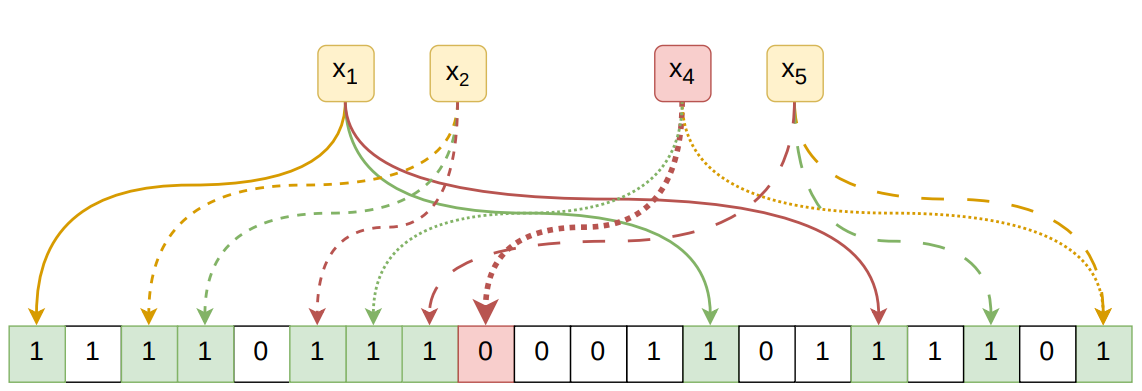
\includegraphics[width=0.5\textwidth]{img/hash/bloom.png}
    \caption{Esempio di query su Bloom Filter}
\end{figure}
\newpage
Una generalizzazione dei Bloom filter sono \textbf{Counting Bloom filter}. In
queste strutture dati si tiene conto anche di quante funzioni di hash mappano in
una certa posizione dato un elemento qualsiasi si verifica la presenza tramite
il counting Bloom filter tramite una threshold $\theta$.

Possiamo costruire questa struttura dati nel seguente modo:
\begin{equation}
    \forall k \in S \ text{e} \ \forall h_i \in \mathcal{H}: A[h_i(k)] += 1
\end{equation}
In fase di query, dato $x \in \mathcal{U}$ abbiamo:
\begin{itemize}
    \item Se $\exists h_i \in \mathcal{H}$ tale che $A[h_i(x)] = 0$ o
          $A[h_i(x)] \leq \theta$ allora $x \notin S$
    \item Se $\forall h_i \in \mathcal{H}$ $A[h_i(x)] > 0$ o $A[h_i(x)] > \theta$
          allora "probabilmente" $x \in S$, avendo $\mathcal{P}(FP) \neq 0$
    \item $A[h_i(x)]$ è una sovrastima del numero di elementi $x$ in $S$.
\end{itemize}
\section{Heavy Hitters Problem}
L'\textbf{heavy hitters problem} consiste nell'identificazione dell'elemento più
frequente o anche detto \textbf{heavy hitter}. Questo problema non può essere
risolto utilizzando un \textbf{Bloom Filter} in quanto richiederebbe troppo spazio
di memorizzazione.
\begin{definizione}[\textbf{Stream di dati}]
    Con \textbf{stream di dati} si intende una sequenza di dati passati uno ad
    uno alla struttura dati. Quindi, data una sequenza $S = s_0,s_1, \dots ,s_{n-1}$,
    prima si considera $s_0$, poi $s_1 \ \dots$ fino a $s_{n-1}$ si costruisce
    quindi una struttura dati che può essere interrogata con nuovi valori
    $x \in \mathcal{U}$.
\end{definizione}
Su questa struttura dati è possibile effettuare le seguenti query:
\begin{itemize}
    \item Quante volte appare $x$ nello stream:
          \begin{equation}
              | \{ i \in \{0, 1, \dots, n - 1\}| \ s_i = x \}|
          \end{equation}
    \item Quanti elementi distinti si hanno nello stream:
          \begin{equation}
              |\{s_i | i \in \{0, 1, \dots, n - 1\}\}|
          \end{equation}
\end{itemize}
\subsection{Count-min sketch}
Una struttura dati che ci permette di risolvere questo problema è il
\textbf{Count-min sketch}, la quale richiede poco spazio in memoria ed è
concettualmente simile a un Bloom filter.

Questa struttura dati è definita a partire da:
\begin{itemize}
    \item Insieme universo $\mathcal{U}$.
    \item Uno stream $S$ lungo $n$ costruito da elementi di $\mathcal{U}$.
    \item Due parametri d'errore $\delta$ e $\varepsilon$. Otterremo risposte
          alle query ``sbagliate'' entro un fattore aggiuntivo $\varepsilon$ con
          probabilità almeno $1 - \delta$
    \item $\mathcal{H}, \ |\mathcal{H}| = l = \lceil \ln \frac{1}{\delta} \rceil$,
          famiglia di funzioni hash universale per $\mathcal{U}$ si impone che:
          \begin{equation}
              h_i: \mathcal{U} \to \{0, \dots, m\}, \ \forall h_i \in \mathcal{H},
              \ \text{con} \ m = \left\lceil \frac{e}{\varepsilon} - 1 \right\rceil
          \end{equation}
\end{itemize}
Il \textbf{Count-min sketch} è costituito da una matrice bidimensionale $T$ con
$l$ righe, una per ogni $h_i \in \mathcal{H}$, e $m$ colonne. Si hanno quindi $l$
hash table indipendenti con $m$ entry ciascuna. La matrice $T$ viene inizializzata
con tutti gli elementi a $0$.

Il caricamento di $T$ avviene nel seguente modo:
\begin{itemize}
    \item Si considerano in ordine tutti gli $x_j \in S$, con $j = 0, 1, \dots,
              n - 1$.
    \item Sappiamo che ogni $h_i$ ha di fatto come codominio l'insieme degli indici
          di colonna. Quindi inserire $x_j$ in T vuol dire incrementare di 1
          $T_{h_i} [h_i(x_j)]$, $\forall h_i \in H$
\end{itemize}
Queste operazioni richiedono un tempo per essere eseguite pari a $\mathcal{O}(n)$,
dove $n$ è la lunghezza dello stream.

Su questa struttura dati è possibile eseguire la query per $q \in \mathcal{U}$
nel seguente modo:
\begin{itemize}
    \item Si applica ogni funzione di hash a $q$
    \item Si tiene traccia di ogni $T_{h_i} [h_i(q)]$, $\forall h_i \in \mathcal{H}$
    \item Si restituisce il minimo tra tali valori, che è una stima (una frequenza
          approssimata $\hat{a}_q$) di quante volte occorre $q$ in $S$:
          \begin{equation}
              \hat{a}_q = \min_{h_i \in \mathcal{H}} T_{h_i} [h_i(q)]
          \end{equation}
\end{itemize}
Una query si effettua in tempo $\mathcal{O}(l)$.

È possibile dimostrare che data $a_q$, ovvero la frequenza reale di $q$ in $S$,
si ha che:
\begin{equation}
    a_q \leq \hat{a}_q
\end{equation}
Si dimostra che $a_q \leq \hat{a}_q$ a causa delle collisioni si ottengono
sovrastime ma mai sottostime della frequenza.

Inoltre, è possibile dimostrare:
\begin{equation}
    \hat{a}_q \leq a_q + \varepsilon \cdot n
\end{equation}
con probabilità almeno $1 - \delta$.

Dato che la matrice bidimensionale $T$ è di dimensione $l \times m = \lceil \ln
    \frac{1}{\delta} \rceil \times \lceil \frac{e}{\varepsilon} \rceil$ con
valori che richiedono $\log n$ bit, allora la struttura dati occupa uno spazio
pari a:
\begin{equation}
    \left( \left\lceil \ln \frac{1}{\delta} \right\rceil \cdot \left\lceil
    \frac{e}{\varepsilon} \right\rceil \cdot \log n \right) \ \text{bit}
\end{equation}
\begin{figure}[!ht]
    \centering
    \begin{subfigure}[b]{0.45\textwidth}
        \centering
        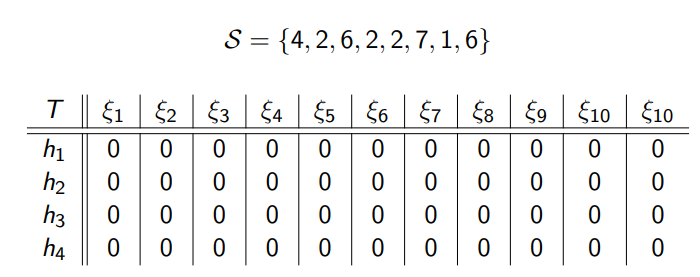
\includegraphics[width=\textwidth]{img/hash/CMS1.png}
        \caption{Inizializzazione}
    \end{subfigure}
    \hfill
    \begin{subfigure}[b]{0.45\textwidth}
        \centering
        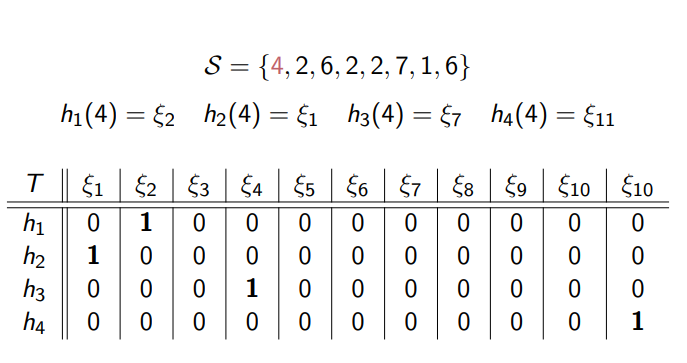
\includegraphics[width=\textwidth]{img/hash/CMS2.png}
        \caption{Inserimento del primo elemento}
    \end{subfigure}
    \hfill
    \begin{subfigure}[b]{0.45\textwidth}
        \centering
        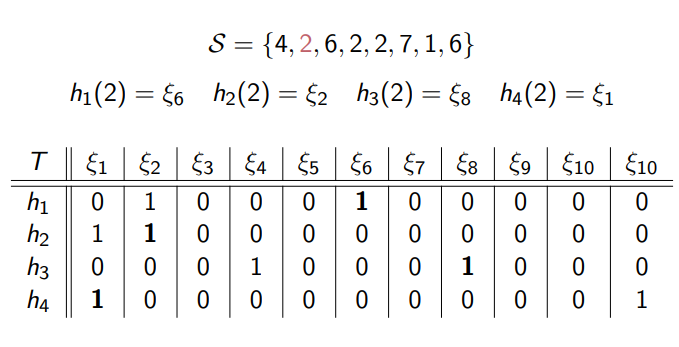
\includegraphics[width=\textwidth]{img/hash/CMS3.png}
        \caption{Inserimento del secondo elemento}
    \end{subfigure}
    \hfill
    \begin{subfigure}[b]{0.45\textwidth}
        \centering
        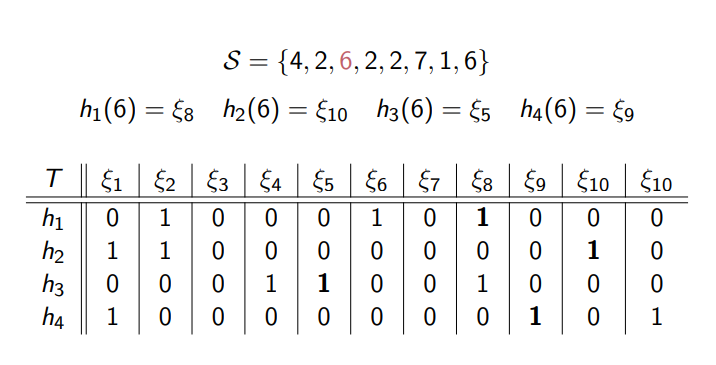
\includegraphics[width=\textwidth]{img/hash/CMS4.png}
        \caption{Inserimento del terzo elemento}
    \end{subfigure}
    \caption{Esempio di riempimento Count-min sketch}
\end{figure}